\chapter{Výsledky}

\section{Testovanie}
Pri testovaní vizualizácie sme postupovali podľa článku od Elmqvist et al. \cite{Patterns}, ktorý opisuje najpoužívanejšie vzory testovania vizualizácie a článok od Vogel et al., v ktorom autori testujú webovú vizualizáciu \cite{WebBasedUserTest}.

\subsection{Testovacia procedúra}
Testovanie prebiehalo prostredníctvom niekoľkých úloh, ktoré sme navrhli na základe špecifikácie požiadaviek na vizualizáciu uvedených v sekcii \ref{sec:spec}. 

Každému subjektu bola predstavená základná funkcionalita systému v krátkom 15 minútovom návode. Následne subjekt obdržal testovací formulár (pozri prílohu \ref{sec:testform}) obsahujúci 7 rôznych úloh, ktoré mal subjekt vykonať a po vykonaní každej z nich do formulára zapísať výsledok svojho skúmania.

Pri testovaní sme jednak vyhodnocovali správnosť odpovedí ale aj rýchlosť vykonania jednotlivých úloh. Taktiež sme dokumentovali interakciu s vizualizáciou počas vykonávania úlohy pomocou \textit{screen capture}.

\subsection{Výsledky testovania}

Vizualizáciu sme testovali na 6 subjektoch bez vyššieho meteorologického, matematického alebo informatického vzdelania. Taktiež žiaden užívateľ nemal skúsenosti s verifikáciou predpovedí a náš systém videl prvýkrát v živote. Všetky tieto faktory vplývali na výsledok nášho testu, keďže sme sa často stretali s nepochopením respektíve s pomalým pochopením zadania a teda čas riešenia úlohy sa značne natiahol.

V tabuľke \ref{table:results} môžme vidieť, že všetci testovaní užívatelia vyriešili všetky úlohy správne a výsledky riešenia sa líšili iba v nameranom čase. V tabuľke je hrubým písmom zvýraznený najdlhší a najkratší priemerný čas pre dané úlohy. 
V priemere každá úloha trvala asi pol minúty (26s) a všetky úlohy užívatelia vykonali v priemere za 3 minúty.


\begin{table}[h]
\centering
\caption{Výsledky testovania}
\label{table:results}
\begin{tabular}{|c|c|c|c|}
\hline
\rowcolor[HTML]{9B9B9B} \textbf{Úloha} & \textbf{Počet správnych} & \textbf{Počet nesprávnych} & \textbf{Priemerný čas} \\ \hline
1              &            6             &             0              &         23.85s                       \\ \hline
2              &            6             &             0              &         37.27s                      \\ \hline
3              &            6             &             0              &         24.66s                      \\ \hline
4              &            6             &             0              &         \textbf{40.36}s                      \\ \hline
5              &            6             &             0              &         24.69s                      \\ \hline
6              &            6             &             0              &         \textbf{9.73}s                      \\ \hline
7              &            6             &             0              &         23.27s                       \\ \hline
\rowcolor[HTML]{C0C0C0} \textbf{Suma}  &           \textbf{42}             &             \textbf{0}              &        \textbf{183.83}                      \\ \hline
\end{tabular}
\end{table}

V grafe na obrázku \ref{fig:results} môžme lepšie vidieť sumárne porovnanie časov pre jednotlivé úlohy a užívateľov. Môžme si ľahko všimnúť, že úlohy 1, 2, 5 a 7 majú približne rovnaký priemerný čas, zatiaľ čo úlohy 2, 4 mali výrazne dlhšie trvanie a úloha 9 trvala v priemere najkratšie.

Dlhé trvanie úlohy 2 prisudzujeme vyššej zložitosti úlohy oproti ostatným. Pre užívateľov bolo odhalenie outlierov pomerne rýchle, avšak väčšinu času zabralo užívateľom odčítanie z grafu o akú presnú hodnotu a predpoveď ide.

Pri úlohe 4 bolo problémom rýchle odčítanie z grafu, o aký dátum sa jedná. Dôvodom bolo nedobré označenie dátumov na \mbox{$ x $-ovej} škále, kedy sa jednotlivé dni v roku označujú číslami 0-364. Užívateľ uvidel konkrétny dátum, až keď nadišiel myšou na dané miesto, kedy sa mu presné hodnoty ukázali v \textit{tooltipe}. Lepším riešením by bola redšia škála s mesačnými intervalmi alebo konkrétnymi dátumami.

Výsledky nášho testovania považujeme celkovo za uspokojivé, keďže aj neskúsení užívatelia dosahovali pri všetkých úlohách dobré časy. Taktiež nám tieto výsledky poukázali na slabiny našej práce, ktorými sú hlavne zlé alebo slabé označenia škál, grafov a legiend.

\begin{figure}
	\centering
	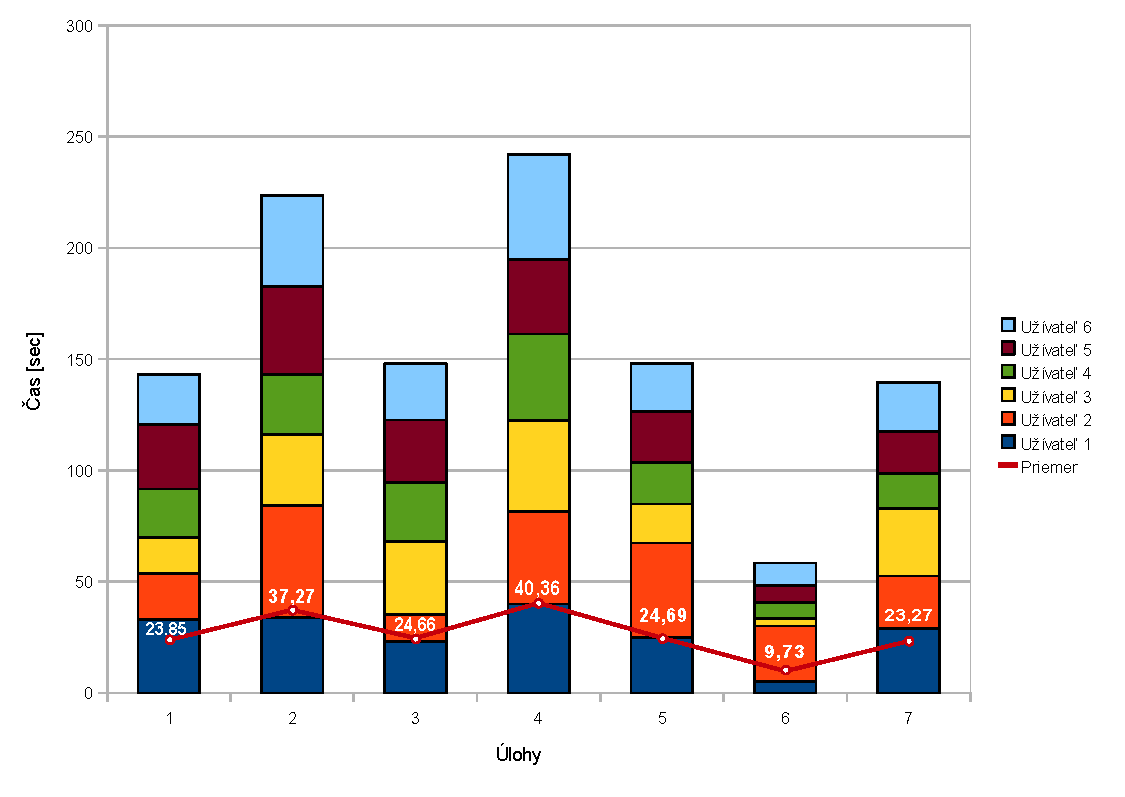
\includegraphics[width = 5in]{resultchart}
	\caption{Výsledky testovania.}
	\label{fig:results} 
\end{figure}

\section{Demonštrácia}
